\section{Momentenregelung des Antriebstranges} \label{regelung}
%Chris
\subsection{Regelungsziele und Regelkreis}
Bevor eine Regelung für die WEA umgesetzt werden kann, müssen zunächst einige Regelungsziele festgelegt werden. Aus der Beschreibung der Regelungsziele ergeben sich die Regelanforderungen der WEA. Des Weiteren wird die Komplexität des Reglers durch ein geeignetes Funktionsmodell, welches das dynamische Verhalten der Regelstrecke bestimmt, beschrieben. Hierfür wird das torsionsstarre Triebstrangmodell verwendet. Die Regelung konzentiert sich auf die Einhaltung und Umsetzung der Hauptziele, wobei das Verhalten der Blätter, des Turms und des Antriebsstranges nicht berücksichtigt wird. Folglich reicht ein sehr vereinfachtes Funktionsmodell aus. Aus der Generatorcharakteristik lassen sich insgesamt drei Arbeitsbereiche ermitteln, nämlich der untere und obere Teillastbereich, sowie der Volllastbereich. Die folgende \autoref{tab:Tabelle4.1} fasst die Hauptziele des Reglers zusammen. Auf Grundlage dessen, werden in den folgenden Kapiteln die benötigten Regler für die verschiedenen Arbeitsbereiche entwickelt.
\\


\begin{table}[H]
    \centering
    \begin{tabular}{|l|}
        \hline                                                        
        \rowcolor{lightGrey}
        \multicolumn{1}{|c|}{ \textbf{Unterer Teillastbereich (I)}}                                                                                                   \\ \hline
    
         Leistungsoptimierung - Leistungsbeiwert \acs{cP} stets auf maximalen Leistungsbeiwert\\ \acs{cPmax} halten.
         \\
         Anforderung: \acs{cP} = \acs{cPmax}
                                   \\ \hline
        \rowcolor{lightGrey}
        \multicolumn{1}{|c|}{\textbf{Oberer Teillastbereich (II)}}                                                                                                      \\ \hline
        Leistungsoptimierung - Leistungsbeiwert \acs{cP} kleiner als maximaler Leistungsbeiwert\\ \acs{cPmax}.
        \\
        Anforderung: \acs{cP} < \acs{cPmax}
                                        \\ \hline
        \rowcolor{lightGrey}
        \multicolumn{1}{|c|}{\textbf{Volllastbereich (III)}}                                                                                                          \\ \hline
        Leistungsbegrenzung - Leistungsbeiwert \acs{cP} für eine konstante Entnahme der \\Nennwindleistung beeinflussen.
        \\
        Anforderung: \acs{cP} \ll \space \acs{cPmax}
        \\ \hline
    \end{tabular}
    \caption{Hauptziele des Reglers für die jeweiligen Arbeitsbereiche}
    \label{tab:Tabelle4.1}
\end{table}

Für die Regelung der WEA wird von einem Standardregelkreis ausgegangen, wie in \autoref{fig:Abbildung4.1} dargestellt. Wobei für den unteren Teillastbereich ein anderes Konzept verwendet wird und an sich keinen Standardregelkreis darstellt, was in Kapitel 4.2 noch genauer beschrieben wird.
\\
Als Stellgröße u eignet sich das Generatormoment \acs{MG} und der Pitchwinkel \acs{ThetaP}. Da die Windgeschwindigkeit nur sehr ungenau messtechnisch erfasst werden kann und ein stochastisches Verhalten aufweist, eignet sich diese Größe als Störgröße z. Hingegen kann die Rotordrehzahl \acs{omegaR} sehr gut messtechnisch erfasst werden, da die Rotorblätter als Anemometer dienen. Daher eignet sich diese Größe gut als Führungs- und Regelgröße w und y. Die Regler- und Streckenübertragungsfunktion werden für den oberen Teillastbereich und Volllastbereich separat mithilfe der Superposition ermittelt. 

\begin{figure}[H]
    \centering
    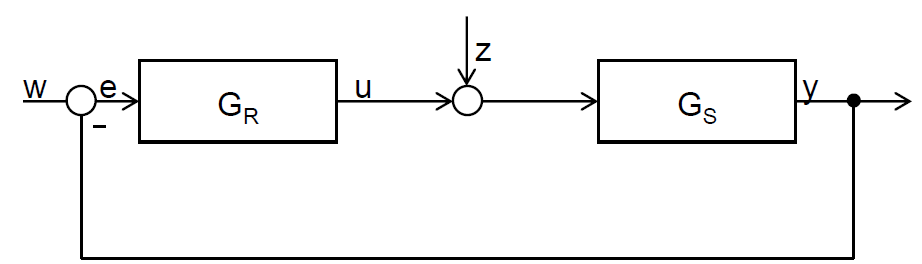
\includegraphics[scale=0.45]{Bilder/Kapitel 6/Standardregelkreis.PNG}
    \caption{Standardregelkreis}
    \label{fig:Abbildung4.1}
\end{figure}

%Chris
\subsection{Unterer Teillastbereich}

Laut \autoref{tab:Tabelle4.1} ist für den unteren Teillastbereich eine Leistungsoptimierung notwendig, da die Windleistung \acs{PW} unterhalb der Generatornennleistung \acs{PG} liegt. Die Rotordrehzahl \acs{nR} liegt folglich noch unter der Generatornenndrehzahl \acs{nG}, wodurch diese noch variabel an die Windgeschwindigkeit \acs{v1} angepasst werden kann. Dies wird mithilfe des bremsend wirkenden Generatormomentes \acs{MG} erreicht. Aufgrund dessen ergibt sich ein optimales Anströmverhältnis und es resultiert ein maximaler Leistungsbeiwert. Im unteren Teillastbereich kann mit steigender Windgeschwindigkeit also die maximal mögliche Windleistung entnommen werden, das heißt, der Leistungsbeiwert \acs{cP} wird stets auf den maximalen Leistungsbeiwert \acs{cPmax} geregelt.
\\
Für die Herleitung des Regelkreises wird von einer nicht linearen Bewegungs-DGL des torsionsstarren Triebstrangs ausgegangen. Der Vorteil für die Reglerauslegung im unteren Teillastbereich besteht darin, dass von der nicht linearen Bewegungs-DGL aus einer Leistungsbilanz ein Regelgesetz abgeleitet wird, welches einen Zusammenhang zwischen Regel- und Stellgröße darstellt. Durch das Regelgesetz wird mithilfe des berechneten Generatormoments \acs{MG} eine stationäre Rotordrehzahl \acs{omegaR} eingestellt. Es wird für diese Methode keine Führungsgröße benötigt. Dies vereinfacht die Entwicklung des Regelkreises für den unteren Teillastbereichs deutlich, da keine genaue Kenntnis der Steckenübertragungsfunktion nötig ist. Daher kann der untere Teillastbereich nicht als Standardregelkreis betrachtet werden. Dieses \glqq Steuerungskonzept\grqq{} zur Regelung des unteren Teillastbereiches hat sich als Standardmethode für diesen Arbeitsbereich durchgesetzt. Das Regelgesetz für die Stellgröße \acs{MG} wird mit folgenden Gleichungen beschrieben:
\newpage

\begin{align}
    \acs{MG}(\acs{omegaG}) = k_I \cdot \acs{omegaR}^2 \enspace ,wobei \enspace \acs{kI} = const.
    \label{eq:Gleichung4.1}
\end{align}

mit:

\begin{align}
   \acs{kI} = \frac{1}{2} \cdot \rho \cdot \pi \cdot R^5 \cdot \frac{1}{\acs{lambdaopt}^3} \cdot \frac{1}{\acs{ng}} \cdot \acs{cP}(\acs{lambdaopt})
   \label{eq:Gleichung4.2}
\end{align}

Der Vorteil bei diesem Steuerungskonzept besteht nun darin, dass für jede Änderung der Windgeschwindigkeit \acs{v1} ein neuer stationärer Arbeitspunkt mit stationärer Rotordrehlzahl \acs{omegaR} entsteht. Dabei ergibt sich ein entsprechendes Generatormoment \acs{MG}, welches mithilfe der \autoref{eq:Gleichung4.1} und \autoref{eq:Gleichung4.2} berechnet werden kann. Das heißt, zu jeder Windgeschwindigkeit wird das zugehörige Generatormoment \acs{MG} zugeordnet, wodurch die Notwendigkeit eines PI(D)-Reglers entfällt.
\\
Die Rotordrehzahl \acs{omegaR} wird stets optimal an die Windgeschwindigkeit angepasst. Es besteht für stationäre Arbeitspunkte ein eindeutiger Zusammenhang zwischen Rotordrehzahl \acs{omegaR} und der Windgeschwindigkeit \acs{v1}. Die optimale Schnelllaufzahl \acs{lambdaopt} kann im voraus berechnet werden und ist für den unteren Teillastbereich konstant. Aufgrund dessen, kann mithilfe der \autoref{eq:Gleichung4.3}, aus der Rotordrehzahl und konstanten Schnelllaufzahl die zugehörige Windgeschwindigkeit \acs{v1} berechnet werden.  Damit ergibt sich für den Leistungsbeiwert \acs{cP} ein optimaler Leistungsbeiwert \acs{cPopt}, jedoch für den Momentenbeiwert \acs{cM} kein optimaler Momentenbeiwert \acs{cMopt}. Aus der Formulierung der Regelziele ergab sich eine Leistungsoptimierung für den unteren Teillastbereich, sodass der Leistungsbeiwert \acs{cP} auf einen optimalen Wert geregelt werden muss, da erst so die maximale Windleistung \acs{PW} entnommen wird. Daher wird das Erreichen eines optimalen Momentenbeiwertes \acs{cMopt} nicht angestrebt, da die Leistungsoptimierung durch Drehzahlanpassung stattfindet.   

\begin{align}
    \acs{v1} = \frac{\acs{omegaR} \cdot {R}}{\acs{lambdaopt}} \enspace ,wobei \enspace \acs{lambda} = \acs{lambdaopt}
    \label{eq:Gleichung4.3}
\end{align}

Die Steuerung für den unteren Teillastbereich wird als Funktionsblock in Matlab Simulink implementiert. In diesem Block wird der Faktor \acs{kI} berechnet und hinterher mit der Rotordrehzahl \acs{omegaR} multipliziert, um als Ergebnis das Generatormoment \acs{MG} zu erhalten, welches als Eingangsparameter für den Antriebstrang dient. Die \autoref{fig:Abbildung4.2} zeigt die Blockdarstellung der Steuerung inklusive der Ein- und Ausgansparameter.

\newpage

\begin{figure}[H]
   \centering
   \begin{pspicture}[showgrid=false](0,0)(10,5)
        \psframe(0,0)(10,5)
        % Modell
        \psframe[linecolor=black,fillcolor=lightGrey,fillstyle=solid](0.5,0.5)(4,4.5)
        \rput(2.25,2.8){\small Steuerung unterer}
        \rput(2.25,2.3){\small Teillastbereich}
        % Ausgänge Block
        \psline{->}(4,2.5)(6,2.5)
        \rput(5.5,2.9){\footnotesize \acs{kI}}
        %Multiplikation
        \psframe[linecolor=black,fillcolor=lightGrey,fillstyle=solid](6.0,0.5)(6.5,4.5)
        \rput(6.25,2.5){\small \cdot}
        % Eingang Multiplikation
        \psline{-}(4.5,4.5)(4.5,3.5)
        \psline{->}(4.5,3.5)(6,3.5)
        \rput(5.3,4.5){\footnotesize {\acs{omegaR}$^2$}}
        % Ausgang Multiplikation
        \psline{->}(6.5,2.5)(9,2.5)
        \rput(8.5,2.9){\footnotesize \acs{MG}}
    \end{pspicture}
   \caption[Übersicht Steuerung unterer Teillastbereich]{Blockdarstellung der Steuerung des unteren Teillastbereichs inklusive der Ein- und Ausgangsparameter}
   \label{fig:Abbildung4.2}
\end{figure}

%Chris
\subsection{Linearisierung der Streckenübertragungsfunktion}
Für die Reglerauslegung im oberen Teillastbereich und Vollastbereich müssen zunächst die Streckenübertragungsfunktionen ausgehend vom torsionsstarren Antriebstrangmodell und der daraus resultierenden nichtlinearen Bewegungs-DGL linearisiert werden. Aus dem Ergebnis der Linearisierung entstehen sogenannte Linearisierungskoeffizienten, welche für einen bestimmten stationären Arbeitspunkt berechnet werden. Für den oberen Teillastbereich und dem Volllastbereich werden zunächst jeweils drei stationäre Arbeitspunkte mit den entsprechenden Linearisierungskoeffizienten betrachtet. Die Linearisierung erfolgt mittels der Taylorreihenentwicklung. Aus dem Funktionsmodell ergibt sich mit \autoref{eq:Gleichung4.4} die nichtlineare Bewegugns-DGL des Antriebstrangs, welche bereits im Kapitel 3 ausführlich diskutiert wurde. 

\begin{align}
    \ddot\varphi_R = \frac{1}{J} \cdot (\acs{MR} - \acs{ng} \cdot \acs{MG})
    \label{eq:Gleichung4.4}
\end{align}

Mithilfe der Taylorreihenentwicklung um einen stationären Arbeitspunkt \acs{omegaR} und lösen der nichtlinearen Bewegungs-DGL mit der Laplacetransformation ergibt sich folgende \autoref{eq:Gleichung4.5}, wobei sich insgesamt vier Linearisierungskoeffizienten ergeben, bei dem der Koeffizient bezogen auf das Generatormoment \acs{MG} nicht benötigt wird und auch nicht weiter aufgeführt wird.

\begin{align}
    \acs{omegaR} &= \frac{1}{J \cdot s - k_{\omega\mathrm{R}}} \cdot (\acs{kv} \cdot v + \acs{ktheta} \cdot \theta - \acs{ng} \cdot \acs{MG})\label{eq:Gleichung4.5}
    \enspace,wobei\\
    k_{\omega\mathrm{R}} &:= (\frac{\delta \acs{MR}}{\delta v})_c , \enspace \acs{kv} := (\frac{\delta \acs{MR}}{\delta \omega\mathrm{R}})_c, \enspace  \acs{ktheta} := (\frac{\delta \acs{MR}}{\delta \theta})_c  \nonumber
\end{align}

Zur Berechnung der Linearisierungskoeffizienten muss nun die Berechnungsvorschrift für das Rotormoment \acs{MR} aus \autoref{eq:Gleichung2.39} partiell abgeleitet werden, wobei der Momentenbeiwert \acs{cM} ebenfalls partiell nach \acs{lambda} und $\theta$ abgeleitet werden muss. Daraus ergeben sich die folgenden Gleichungen.

\begin{align}
    k_{\omega\mathrm{R,II(I),i}} &\approx (\frac{1}{2} \cdot \rho \cdot \acs{v1}^2 \cdot \pi \cdot \acs{R}^3 \cdot (\frac{\acs{R}}{\acs{v1}} \cdot \frac{\delta \acs{cM}_{,II(I),i}(\acs{lambda}(v,\acs{omegaR}),\theta)}{\delta \acs{lambda}}))_c\label{eq:Gleichung4.6}\\
     \acs{kv}_{,II(I),i} &\approx (\frac{1}{2} \cdot \rho \cdot \acs{v1}^2 \cdot \pi \cdot \acs{R}^3 \cdot (2 \cdot \acs{v1} \cdot \acs{cM}_{,II(I),i}(\acs{lambda}(v,\acs{omegaR}),\theta) - \acs{omegaR} \cdot \acs{R} \cdot \frac{\delta \acs{cM}_{,II(I),i}(\acs{lambda}(v,\acs{omegaR}),\theta)}{\delta \acs{lambda}}))_c\label{eq:Gleichung4.7}\\
    \acs{ktheta}_{,III,i} &\approx (\frac{1}{2} \cdot \rho \cdot \acs{v1}^2 \cdot \pi \cdot \acs{R}^3 \cdot (\frac{\delta \acs{cM}_{,III,i}(\acs{lambda}(v,\acs{omegaR}),\theta)}{\delta \acs{lambda}}))_c\label{eq:Gleichung4.8}
\end{align}

Im Folgenden werden die weiteren nötigen Schritte aufgeführt, um die Berechnung der Linearisierungskoeffizienten zu vervollständigen. Zunächst werden die Schnelllaufzahlen \acs{lambda} für die Arbeitsbereiche und dessen stationäre Arbeitspunkte mit der \autoref{eq:Gleichung4.9} berechnet.

\begin{align}
    \acs{lambda}_{,II(I),i} = \frac{\acs{omegaR} \cdot R}{\acs{v1}_{,II(I),i}}
    \label{eq:Gleichung4.9}
\end{align}

Hinterher werden die partiellen Ableitungen der Momentenbeiwerte \acs{cM} mithilfe der \autoref{eq:Gleichung4.10} und Unterscheidung der Arbeitsbereiche berehcnet. Für den oberen Teillastbereich muss die partielle Ableitung nach $\theta$ nicht erfolgen, da der Pitchwinkel hier null beträgt. Der Pitchwinkel wird erst beim Volllastbereich von Bedeutung sein, wenn es darauf ankommt, die Rotordrehzahl \acs{nR} mithilfe des Pitchwinkels zu begrenzen.

\begin{align}
    \acs{cM}(\acs{lambda})_{,II(I),i,\theta} &= c_1 \cdot (1 + c_2 \cdot \sqrt{\theta + c_3}) + \frac{c_4}{\acs{lambda}}   \cdot (c_5 \cdot \acs{lambda}_i - c_6 \cdot \theta - c_7 \cdot \theta^{c_8} - c_9) \cdot e^{-c_{10} \cdot \acs{lambda}_i}
    \label{eq:Gleichung4.10}\\\enspace ,mit\nonumber\\
    \acs{lambda}_i &= \frac{1}{\acs{lambda}_{,II(I),i} + 0,008 \cdot \theta} - \frac{0,035}{c_{11} + c_{12} \cdot \theta^3}
    \nonumber
\end{align}

{\renewcommand{\arraystretch}{2}%
\begin{table}[H]
    \centering
    \begin{tabular}{|c|c|c|c|}
        \hline
        c$_1$ = 0,005 & c$_2$ = 1,53 & c$_3$ = 0,5 & c$_4$ = 0,18\\\hline
        c$_5$ = 121 & c$_6$ = 27,9 & c$_7$ = 198 & c$_8$ = 2,36\\\hline
        c$_9$ = 5,74& c$_{10}$ = 11,35 & c$_{11}$ = 16,1 & c$_{12}$ = 201\\\hline
    \end{tabular}
\end{table}
}
\newpage

Die Berechnung der Schnelllaufzahlen \acs{lambda}$_{,II(I),i}$ für den jeweiligen Arbeitsbereich und dessen stationären Arbeitspunkte, die Berechnung der partiellen Ableitungen für die Momentenbeiwerte \acs{cM}$_{,II(I),i}$, sowie die Berechnung der Linearisierungskoeffizienten und dessen partielle Ableitungen, finden in einem separaten Matlab-File statt und werden bevor die Simulation gestartet wird vorangehend einmalig für die stationären Arbeitspunkte berechnet und für die Berechnung der Reglerkoeffizienten für den oberen Teillastbereich und Volllastbereich zur Verfügung gestellt, welche ebenfalls vor Simulationsstart einmalig berechnet werden und hinterher als Array der Simulation übergeben und in entsprechende Lookup Tables gespeichert.
% HI :)
%chris + Aaron
\subsection{Oberer Teillastbereich}
%Einleitung für das Kapitel in Vorlesungsfolie "Einführung in die WEA Regelung" Seite 55
Laut \autoref{tab:Tabelle4.1} ist für den oberen Teillastbereich ebenfalls eine Leistungsoptimierung notwendig, da die Windleistung \acs{PW} noch unterhalb oder gleich der Generatornennleistung \acs{PG} ist. Sofern die Rotordrehzahl \acs{nR} gleich der Generatornenndrehzahl \acs{nG} ist, ist es nicht mehr möglich diese an die Windgeschwindigkeit anzupassen. Dadurch ergibt sich ein schlechtes Anströmverhältnis was einen nicht optimalen Leistungsbeiwert \acs{cP} zur Folge hat. Es wird zwar nicht mehr das Leistungsmaximum aus der zur Verfügung stehenden Windleistung entnommen, dennoch wird eine Leistungssteigerung mit ansteigender Windgeschwindigkeit \acs{v1} durch eine geeignete Regelung erzielt. 

%Chris + Aaron
\subsection{Volllastbereich}
%Einleitung für das Kapitel in Vorlesungsfolie "Einführung in die WEA Regelung" Seite 56

Laut \autoref{tab:Tabelle4.1} ist für den Volllastbereich eine Leistungsbegrenzung vorzusehen, da nun die Windleistung \acs{PW} oberhalb der Generatornennleistung \acs{PG} liegt. Durch das Pitchen der Blätter wird bewusst das Anströmverhältnis verschlechtert, denn die WEA ist nicht in der Lage weit über Nenndrehzahl beschleunigt zu werden. Dies würde zur Beschädigung oder gar Zerstörung der WEA führen. Das Pitchen ermöglicht jedoch bei ansteigender Windleistung (\acs{PW} > \acs{PG}) weiterhin eine konstante Generatornennleistung \acs{PG} zu erzeugen. Der Pitchwinkel \acs{ThetaP} spielt nun für die Reglerauslegung eine entscheidene Rolle.   

